\section{Appendix}

\subsection{Computation of DeepGeo's \textit{effective dimensionality}}
\label{ch5:sec:appendix_effe_dim}

To quantify the \textit{effective dimensionality} of DeepGeo, we use the approach described in \citet{ai.Maddox2020}. In this framework, \textit{effective dimensionality} is computed using the eigenvalues $\{\lambda_1,\lambda_2,...,\lambda_K\}$ of a symmetry matrix--the Hessian of DeepGeo's weights $\textbf{H}_W$, defined as
\begin{equation}
    N_{eff}(\textbf{H}_W) = \sum_{i=1}^K \frac{\lambda_i}{\lambda_i+z}\;,
    \label{ch5:eq:response_effective_dimensionality}
\end{equation}
where $z=10^{-3}$ is a regularization constant. 

Instead of calculating a single large Hessian for all parameters, we compute the Hessian separately for each fully connected layer (layers 1–3 and the output layer). This layer-wise computation not only reduces the computational burden but also provides clearer insight into how each layer contributes to the overall \textit{effective dimensionality}.
For each layer, the Hessian matrix is obtained using Pytorch's auto-differentiation. The overall value is computed as a weighted sum of each layer's \textit{effective dimensionality}, with weights corresponding to the parameter ratio of that layer in DeepGeo. For random DeepGeo models, the \textit{effective dimensionality} is computed with 20 repeated random initializations. This methodology provides a more in-depth view of how DeepGeo utilizes over-parameterization through its initialization.

% !TEX root = ../main.tex
% !TEX spellcheck = en-US

\begin{figure}[tbh]
    \begin{center}
        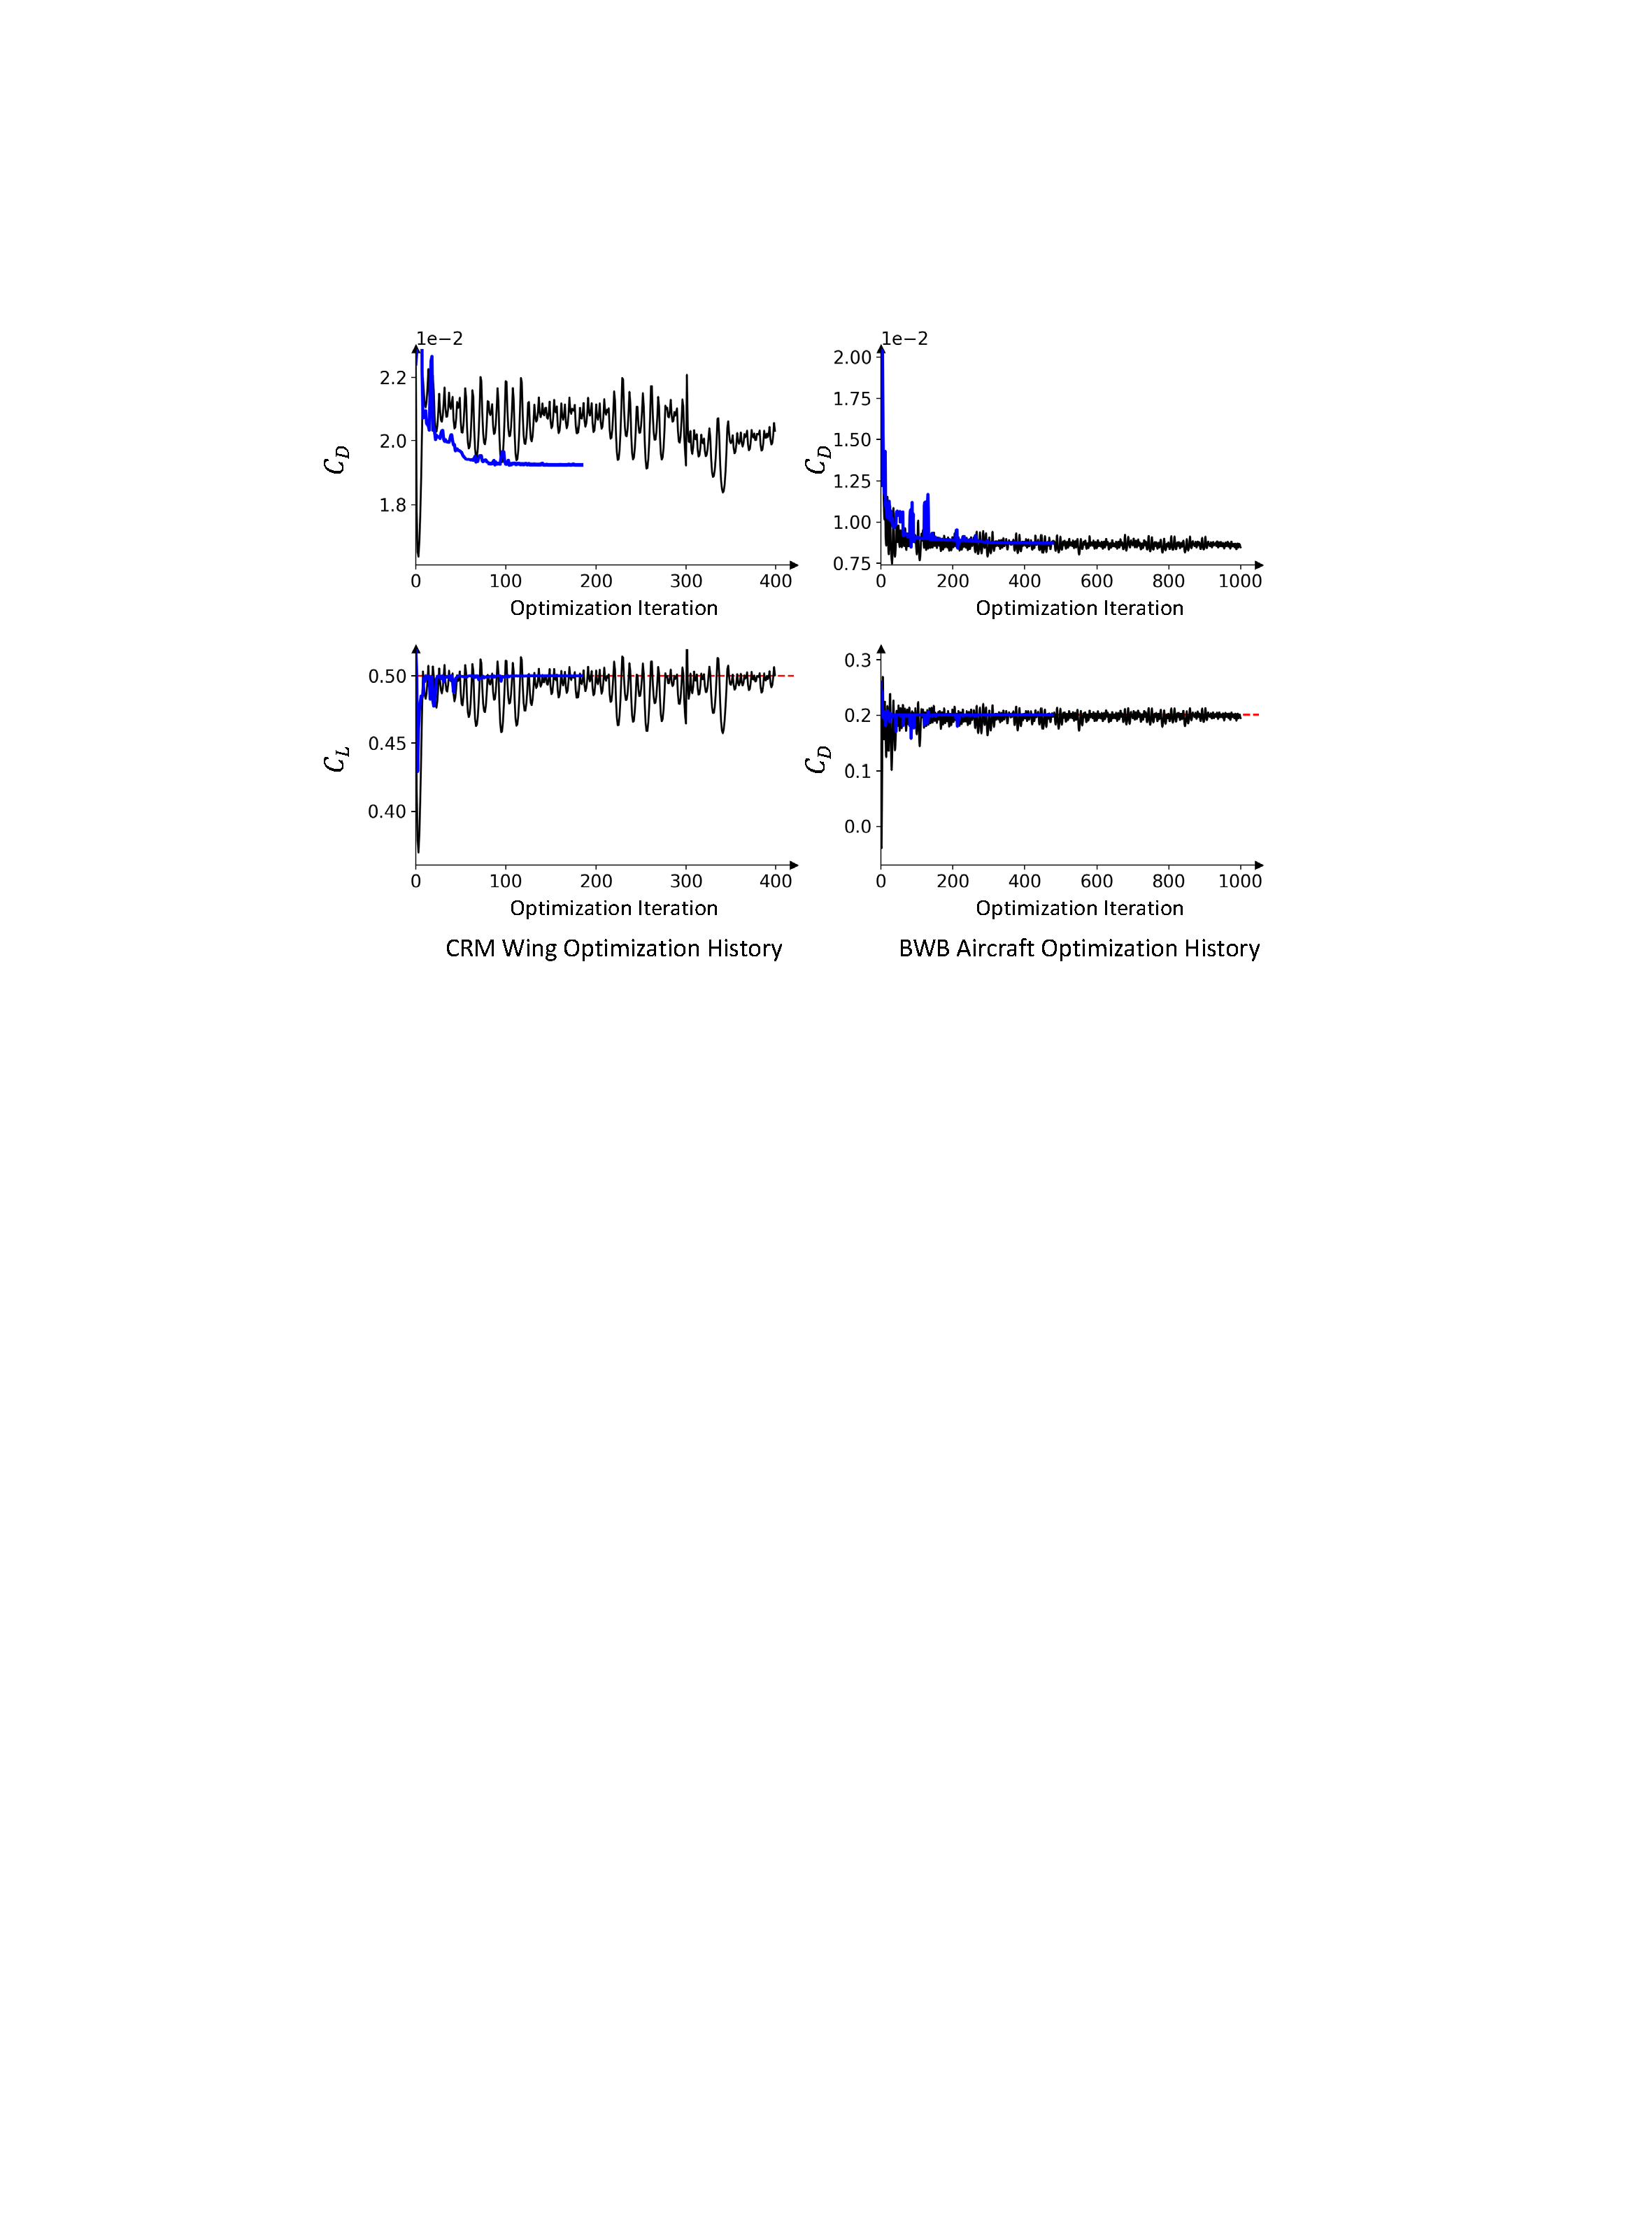
\includegraphics[width=1\linewidth]{chapter5/fig/ffd_history_comparison.pdf}
    \end{center}
    \vspace{-3mm}
    \caption{
        \small The comparison of DeepGeo-based (black) and FFD-based (blue) optimization convergence histories.
    }
    \label{ch5:fig:ffd_history_comparison}
\end{figure}

\subsection{Comparison with FFD-Based Optimization Convergence History}
\label{ch5:sec:appendix_optim_history}

Figure~\ref{ch5:fig:ffd_history_comparison} shows the convergence histories for optimizations with both FFD and DeepGeo. The CRM wing case uses 192-point FFD configuration, while the BWB aircraft case uses 240 control points. Both FFD-based optimizations use the IPOPT optimizer.

The FFD-based optimizations, as shown in blue lines, converge faster than the DeepGeo-based ones, though the number of iterations remains within the same order of magnitude. DeepGeo can achieve significant improvement at early stage, but requires more iterations to reach better optima. For example, in the BWB aircraft case, the DeepGeo-based optimization achieves a shock-free design by the 149th iteration, but continued to improve and reached higher performance after 998 iterations. DeepGeo's convergence path can be less stable due to the inefficient first-order gradient descent optimizer. We believe that further investigation into more advanced optimization strategies could improve DeepGeo's convergence behavior.